\section{Analyser la coh\'erence de cache}
\label{fr:sec:analyze}
Cette section présente les analyses permettant d'utiliser le modèle de
la section précédente pour mettre en évidence les interférences liées
à la cohérence de cache. Une partie de ces travaux ont été publiés
dans \cite{ecrts19}.

\begin{figure}[hbt]
  \centering
  \resizebox{.7\linewidth}{!}{

\begin{tikzpicture}[->,>=stealth',shorten >=1pt,auto,  semithick, node distance=0.5cm]
\tikzstyle{section} = [state, rectangle, fill=gray!20]
\tikzstyle{result} = [state, rectangle, rounded corners]
\tikzstyle{auxresult} = [state,rectangle,draw=white]
\tikzstyle{input} = [state,rectangle, draw=blue, thick, fill=blue!20, align=center, rounded corners, minimum height=2em]
\tikzstyle{interresult} = [state, rectangle,dashed, rounded corners]

\node[section] (WCETANA)
   {
      \begin{tabular}{@{}c@{}}
         WCET\\
         Analysis\\
         (Section~\ref{fr:sec:analysis:wcet})
      \end{tabular}
   };


\node[auxresult] (SLOWFACTOR) [above right=of WCETANA,yshift=-20pt]
   {
      \begin{tabular}{@{}c@{}}
         Slowdown\\
         Factors
      \end{tabular}
   };

\node[result] (PROGWCET) [below right=of WCETANA,yshift=20pt]
   {
      \begin{tabular}{@{}c@{}}
         WCET of\\
         Programs
      \end{tabular}
   };


\node[interresult,node distance=2cm] (NOSHAREDWCET) [below =of WCETANA]
   {
      \begin{tabular}{@{}c@{}}
         Without Shared\\
         Variables
      \end{tabular}
   };

\node[result] (IMPACTWCET) [xshift=-1cm,yshift=-0.5cm, below right =of NOSHAREDWCET]
   {
      \begin{tabular}{@{}c@{}}
         Impact of\\
         Interference\\
         on WCET
      \end{tabular}
   };

\node[section,node distance=4cm] (HITMISSANA) [right =of WCETANA]
   {
      \begin{tabular}{@{}c@{}}
         Hit \& Miss\\
         Analysis\\
         (Section~\ref{fr:sec:cat_cache_access})
      \end{tabular}
   };

\node[input] (PARAMEDMODEL) [above =of HITMISSANA]
   {
      \begin{tabular}{@{}c@{}}
         Instantiated\\
         Model
      \end{tabular}
   };

\node[result] (INSTRACCU) [below left =of HITMISSANA,xshift=1cm]
   {
      \begin{tabular}{@{}c@{}}
         Instruction\\
         Accuracy
      \end{tabular}
   };

\node[auxresult] (MEMEACCU) [below right =of HITMISSANA,xshift=-1cm]
   {
      \begin{tabular}{@{}c@{}}
         Mem. Element\\
         Accuracy
      \end{tabular}
   };


\node[section] (INTERCAT) [right =of HITMISSANA,xshift=2.5cm]
   {
      \begin{tabular}{@{}c@{}}
         Interference\\
         Categorization\\
         (Section~\ref{fr:sec:analysis:exposing_interference})
      \end{tabular}
   };

\node[input] (PROTOCOL) [above =of INTERCAT]
   {
      \begin{tabular}{@{}c@{}}
         Cache Coherence\\
         Protocol
      \end{tabular}
   };

\node[interresult] (ANOTPROTO) [below =of INTERCAT]
   {
      \begin{tabular}{@{}c@{}}
         Annotated\\
         Protocol
      \end{tabular}
   };

\node[section] (INSTRIMPA) [below =of ANOTPROTO,xshift=-0.5cm]
   {
      \begin{tabular}{@{}c@{}}
         Instruction Impact\\
         Analysis\\
         (Section~\ref{fr:sec:analysis:missing_link})
      \end{tabular}
   };

\node[result] (RELINSTRINTER) [below =of INSTRIMPA]
   {
      \begin{tabular}{@{}c@{}}
         Relation Between\\
         Instruction \&\\
         Interference
      \end{tabular}
   };

\path[draw,->] (PARAMEDMODEL) -| (WCETANA);
\path[draw,->] ([yshift=-30pt]WCETANA) -- (PROGWCET);
\path[draw,->] ([yshift=30pt]WCETANA) -- (SLOWFACTOR);

\path[draw,->] (PARAMEDMODEL) -- (HITMISSANA);
\path[draw,->] (HITMISSANA) -- (INSTRACCU);
\path[draw,->] (HITMISSANA) -- (MEMEACCU);

\path[draw,->] (PROTOCOL) -- (INTERCAT);
\path[draw,->] (INTERCAT) -- (ANOTPROTO);
\path[draw,->] (ANOTPROTO) -- (INSTRIMPA);
\path[draw,->] (PARAMEDMODEL) -| ([xshift=10pt]INSTRIMPA.north west);
\path[draw,->] (INSTRIMPA) -- (RELINSTRINTER);

\path[draw,->] ([xshift=-20pt]WCETANA) -- ([xshift=-20pt]NOSHAREDWCET);
\path[draw,->] (PROGWCET) -- (IMPACTWCET);
\path[draw,->] (NOSHAREDWCET) -- (IMPACTWCET);
\end{tikzpicture}
}
\caption{Vue d'ensemble des analyses proposées}
\label{fr:fig:analysis:summary}
\end{figure}

Le modèle présenté dans la section précédente comporte des paramètres (par exemple la durée d'un accès à la mémoire) qui doivent être instanciés via une campagne de benchmarks afin de mener les analyses qui sont décrites ici. Ce processus d'instanciation est en dehors du périmètre de la thèse.
La Figure~\ref{fr:fig:analysis:summary} fournit une vue d'ensemble des analyses
proposées. Les rectangles avec fond gris correspondent aux analyses et ceux sans
arrière plan sont les résultats principaux. Les éléments sans bordure sont des
résultats accessoires. Les bordures en pointillés indiquent les résultats
intermédiaires, qui ne sont pas censés être utiles en eux-mêmes.

% Pour que les analyses présentées dans cette section fournissent des informations
% intéressantes à l'applicant, le modèle doit être instancié afin de correspondre
% à l'architecture cible. Cela signifie que les paramètres listés dans
% l'Annexe~\ref{app:model_parameters} ont été définis suite
% à une campagne de benchmarks mesurant la performance.

\begin{figure}[hbt]
\begin{minipage}[c]{0.55\linewidth}
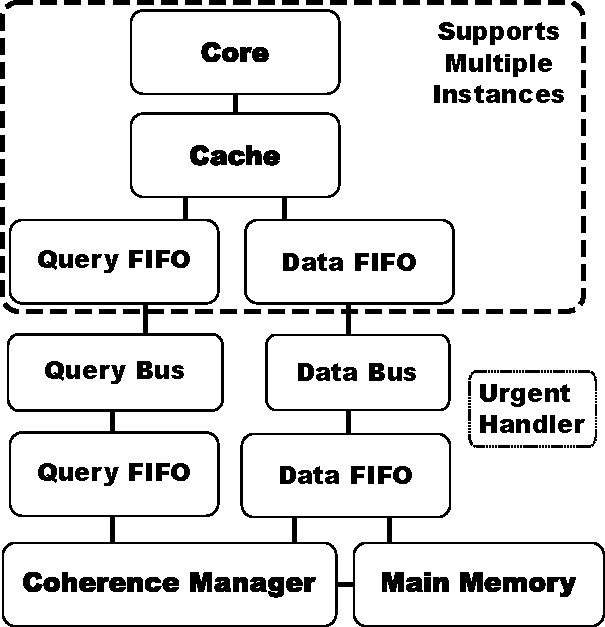
\includegraphics[width=\linewidth]{\chapterdirectory/figure/analysis/model_overview.pdf}
\caption{Aperçu de l'exemple de modèle instancié}
\label{fr:fig:analysis:model}
\end{minipage}
\begin{minipage}[t]{0.2\linewidth}
\begin{enumerate}
  \setlength{\itemsep}{0pt}%
   \setlength{\parskip}{0pt}%
\item \texttt{store 1}
\item \texttt{store 2}
\item \texttt{load 1}
\item \texttt{store 1}
\item \texttt{load 3}
\item \texttt{store 2}
\item \texttt{load 1}
\item \texttt{store 1}
\item \texttt{load 2}
\item \texttt{store 2}
\item \texttt{end}
\end{enumerate}
\caption{Modèle de programme pour Cœur 1}
\label{fr:fig:analysis:demo_prog1}
\end{minipage}
\begin{minipage}[t]{0.2\linewidth}
\begin{enumerate}
  \setlength{\itemsep}{0pt}%
   \setlength{\parskip}{0pt}%
\item \texttt{store 1}
\item \texttt{store 3}
\item \texttt{load 3}
\item \texttt{store 2}
\item \texttt{load 1}
\item \texttt{store 2}
\item \texttt{load 3}
\item \texttt{store 1}
\item \texttt{load 2}
\item \texttt{store 3}
\item \texttt{end}
\end{enumerate}
\caption{Modèle de programme pour Cœur 2}
\label{fr:fig:analysis:demo_prog2}
\end{minipage}
\end{figure}

Le modèle instancié utilisé pour l'illustration des analyses dans cette section
est représenté dans la Figure~\ref{fr:fig:analysis:model}. Celui-ci utilise un
protocole MESI dont les détails sont fournis dans la version complète de la
thèse (voir Figure~\ref{fig:mesi_cc_table}). Le programme
utilisé par chaque cœur est indiqué par les
Figures~\ref{fr:fig:analysis:demo_prog1} et \ref{fr:fig:analysis:demo_prog2}.
Ces modèles instanciés comportent toujours de l'indéterminisme, qui
représente ce que l'applicant ne connaît pas ou ne peut pas contrôler
sur l'architecture.  Par conséquent, le modèle instancié admet
toujours plusieurs traces d'exécution possibles. Les analyses étant
basées sur l'algorithme de model checking d'UPPAAL, toutes ces traces
sont explorées.


\subsection{Analyse de l'impact sur le temps d'exécution}
\label{fr:sec:analysis:wcet}
Cette première analyse regarde les effets de l'interférence sur le temps
d'exécution total des programmes. Notons cependant qu'il s'agit du temps d'exécution calculé sur le modèle
qui peut s'éloigner du temps d'exécution sur l'architecture réelle, notamment en raison des abstractions faites dans la modélisation ou d'une instanciation du modèle insuffisamment précise. 
Les valeurs obtenues sont tout de même intéressantes à comparer avec
d'autres analyses de temps sur un modèle similaire, par exemple pour
le calcul de facteurs de ralentissement (voir
Définition~\ref{fr:def:slowdownfactor}). Par exemple, on peut obtenir
la proportion du temps d'exécution causée par la cohérence de cache en
comparant le modèle avec une version adaptée du même modèle dans laquelle
aucune variable n'est partagée. Bien que cette version adaptée ne soit
probablement pas réaliste, son temps d'exécution peut être utilisé
comme point de référence.

\begin{definition}[Impact de la cohérence de cache sur le temps d'exécution]
Soit $W_{s}$ le temps d'exécution d'un programme sur le modèle instancié, et
$W_{p}$ son temps d'exécution sur une instance du même modèle dans laquelle
toutes les variables ont été rendues privées. La part de $W_{s}$ correspondant
aux mécanismes de cohérence de cache peut être obtenue avec l'équation suivante:
$T_{cc} = W_{s} - W_{p}$
\end{definition}

Pour obtenir les valeurs de $W_{s}$ et $W_{p}$ en utilisant UPPAAL, on emploie
la vérification de modèle. En effet, ces valeurs correspondent au maximum d'une
horloge mesurant le temps d'exécution du cœur étudié. Il est donc possible de la
récupérer avec une formule semblable à\\
\lstinline!sup{not Core1.Terminated}: Core1.runtime!, qui retourne le maximum
pour l'horloge \lstinline!Core1.runtime! dans l'ensemble des états du système
pour lesquels l'automate \lstinline!Core1! n'est pas dans la localité
\lstinline!Terminated!.

\begin{example}[Exemple de mesures de temps d'exécution]
\begin{figure}[hbt]
\centering
\begin{tabular}{|c|c|c|c|c|}
\cline{2-5}
\multicolumn{1}{c|}{}
      & $W_s$ & $W_p$ & $T_{cc}$ & Isolation \\
\hline
Cœur 1 & 2652 & 1102 & 1550 & 702\\
\hline
Cœur 2 & 2452 & 1452 & 1000 & 904\\
\hline
\end{tabular}
\caption{Exemple d'analyse de temps d'exécution}
\label{fr:fig:analysis:wcet_calc}
\end{figure}
La Figure~\ref{fr:fig:analysis:wcet_calc} indique la valeur maximale du temps
d'exécution pour chaque cœur, avec différentes versions de l'exemple du modèle
instancié.
$W_s$ correspond à celle du modèle instancié original (et donc avec les
variables partagées). $W_p$ correspond à celle d'un modèle dans lequel toutes les
variables ont été rendues privées. Ici, on incrémente les adresses d'éléments
mémoires du programme sur le Cœur 2 par $3$ pour éviter tout partage. $T_{cc}$
correspond à la part du temps d'exécution de $W_s$ prise par les mécanismes de
cohérence cache. Enfin, pour montrer un exemple de facteur de ralentissement, on
étudie aussi le cas où chaque programme est exécuté en isolation.
Les résultats de l'analyse sont donc:
\begin{itemize}
    \setlength{\itemsep}{0pt}%
   \setlength{\parskip}{0pt}%
\item
   Cœur 1 souffre d'un facteur de ralentissement de $2652/702 = 3,77$ quand son
   programme tourne en même temps que celui de Cœur 2, comparé à son exécution
   en isolation.
\item
   Cœur 2 souffre d'un facteur de ralentissement de $2452/904 = 2,71$ quand son
   programme tourne en même temps que celui de Cœur 1, comparé à son exécution
   en isolation.
\item
   Exécuter les deux programmes en isolation l'un après l'autre aurait un temps
   d'exécution maximum de $702 + 904 = 1606$ unités de temps.
\item
   Exécuter les deux programmes en parallèle a un temps d'exécution maximal de
   $\max(2652, 2452) = 2652$.
\item
   Exécuter les deux programmes en parallèle mais sans variables partagées a un
   temps d'exécution maximal de $\max(1102, 1452) = 1452$.
\item
   Approximativement $(1550/2652)*100=58,44 \%$  du temps d'exécution de
   Cœur 1 est causé par l'interférence liée à la cohérence de caches.
\item
   Approximativement $(1000/2452)*100=40,78\%$ du temps d'exécution de
   Cœur 2 est causé par l'interférence liée à la cohérence de caches.
\end{itemize}
\end{example}


\subsection{Catégorisation des accès au cache}
\label{fr:sec:cat_cache_access}
Une interférence peut empêcher une instruction de récupérer une valeur dans le cache (parce que son contenu a été modifié récemment à cause d'une autre instruction). C'est ce qu'on appelle un \emph{cache-miss}.
Les analyses de cette
section s'intéressent à la catégorisation des instructions en fonction des \emph{cache-miss} observés. C'est une technique utilisée dans la littérature (voir
Section~\ref{fr:sec:handling_it}).
L'objectif de cette analyse est donc de classer chaque instruction en
tant que \textit{always-hit} (cache toujours prêt),
\textit{always-miss} (cache jamais prêt) ou \textit{uncategorized} (le
cache peut être prêt ou ne pas l'être selon l'exécution). Pour cela,
on utilise l'opérateur de logique temporelle \agop{} afin de s'assurer
que pour toute trace d'exécution du modèle, l'instruction donnée:
\begin{itemize}
    \setlength{\itemsep}{0pt}%
   \setlength{\parskip}{0pt}%
\item Est résolue par le cache immédiatement, dans quel cas l'instruction est
classée \textit{always-hit}.
\item N'est pas résolue par le cache immédiatement et donc
classée \textit{always-miss}.
\item Sinon, on la classe comme \textit{uncategorized}.
\end{itemize}

\begin{example}[Catégorisation des accès au cache]
\label{fr:ex:analysis:instr_chara}
\begin{figure}[hbt]
\begin{center}
\begin{subfigure}[t]{0.45\textwidth}
\centering
\begin{enumerate}
    \setlength{\itemsep}{0pt}%
   \setlength{\parskip}{0pt}%
\item \texttt{store 1} est classé \texttt{AM}.
\item \texttt{store 2} est classé \texttt{AM}.
\item \texttt{load 1} est classé \texttt{UN}.
\item \texttt{store 1} est classé \texttt{UN}.
\item \texttt{load 3} est classé \texttt{AM}.
\item \texttt{store 2} est classé \texttt{AM}.
\item \texttt{load 1} est classé \texttt{AH}.
\item \texttt{store 1} est classé \texttt{AM}.
\item \texttt{load 2} est classé \texttt{UN}.
\item \texttt{store 2} est classé \texttt{UN}.
\end{enumerate}
\caption{Catégorisation pour le Cœur 1}
\label{fr:fig:analysis:demo_chara_prog1}
\end{subfigure}
\begin{subfigure}[t]{0.45\textwidth}
\centering
\begin{enumerate}
    \setlength{\itemsep}{0pt}%
   \setlength{\parskip}{0pt}%
\item \texttt{store 1} est classé \texttt{AM}.
\item \texttt{store 3} est classé \texttt{AM}.
\item \texttt{load 3} est classé \texttt{AH}.
\item \texttt{store 2} est classé \texttt{AM}.
\item \texttt{load 1} est classé \texttt{AM}.
\item \texttt{store 2} est classé \texttt{UN}.
\item \texttt{load 3} est classé \texttt{AH}.
\item \texttt{store 1} est classé \texttt{AM}.
\item \texttt{load 2} est classé \texttt{UN}.
\item \texttt{store 3} est classé \texttt{AM}.
\end{enumerate}
\caption{Catégorisation pour le Cœur 2}
\label{fr:fig:analysis:demo_chara_prog2}
\end{subfigure}
\end{center}
\caption{Exemple de catégorisation des accès cache}
\label{fr:fig:analysis:demo_chara_progs}
\end{figure}
La Figure~\ref{fr:fig:analysis:demo_chara_progs} montre le résultat de la
catégorisation de chaque instruction de notre exemple.
\texttt{AH} correspond à \textit{always-hit}, \texttt{AM} correspond
à \textit{always-miss} et \texttt{UN} correspond
à \textit{uncategorized}.
\end{example}

Cette catégorisation des instructions permet de déterminer quelles
instructions font varier le temps d'exécution. Cependant, certaines de ces
variations ne sont pas liées à la cohérence de cache. Pour
pouvoir répondre au besoin de la certification, il va donc être
nécessaire d'analyser l'interférence elle-même.

\subsection{Catégorisation de l'interférence}
\label{fr:sec:analysis:exposing_interference}
Pour pouvoir comprendre la cause et les effets des interférences générées par
la cohérence de cache, nous proposons de les classifier en fonction de leurs effets
sur le cache affecté. Cette section présente les trois catégories
d'interférences proposées dans cette thèse.

\begin{definition}[Interférence mineure]
On considère qu'un cache subit une interférence mineure lorsqu'il reçoit une
demande en provenance d'un autre cache sans que cette demande ne nécessite
d'actions de sa part. En effet, le cache a alors pris le temps de traiter une
demande sans que cela n'ait eu d'utilité.
\end{definition}

\begin{example}[Interférence mineure]
Le protocole MSI simplifié de la Section~\ref{fr:sec:cache_coherence_msi}
présente des interférences mineures lorsqu'un cache tenant un élément mémoire
dans l'état \texttt{I} reçoit des demandes, ou qu'il reçoit un \texttt{GetS}
(demande d'accès en lecture) alors qu'il a l'élément en \texttt{S}.
\end{example}

\begin{definition}[Interférence de rétrogradation]
On considère qu'un cache subit une interférence de rétrogradation lorsqu'il
perd les permissions d'écriture sur un élément mémoire suite à la demande d'un
autre cache.
\end{definition}

\begin{example}[Interférence de rétrogradation]
Le protocole MSI simplifié de la Section~\ref{fr:sec:cache_coherence_msi}
présente une interférence de rétrogradation lorsqu'un cache tenant un élément
mémoire dans l'état \texttt{M} reçoit une demande \texttt{GetS} de la part d'un
autre cache. En effet, il passe alors à l'état \texttt{S} et perd ses
permissions d'écriture.
\end{example}

\begin{definition}[Interférence d'expulsion]
On considère qu'un cache subit une interférence d'expulsion lorsqu'il perd
toutes ses permissions sur un élément mémoire suite à la demande d'un autre
cache.
\end{definition}

\begin{example}[Interférence d'expulsion]
Le protocole MSI simplifié de la Section~\ref{fr:sec:cache_coherence_msi}
présente des interférences d'expulsion losrqu''un cache tenant un élément mémoire
dans l'état \texttt{S} ou \texttt{M} reçoit une demande \texttt{GetM} (demande
d'accès en lecture et écriture) de la part d'un autre cache. En effet, il passe
alors à l'état \texttt{I} et perd toutes ses permissions.
\end{example}

\subsection{Révéler les interférences liées à la cohérence de cache}
\label{fr:sec:analysis:missing_link}
Pour révéler toutes les interférences causées par la cohérence de
cache en tenant compte des effets catégorisés, il suffit de
faire en sorte que le modèle détecte les cas où l'interférence a
affecté une instruction. Cela permet alors d'utiliser les outils de
model checking d'UPPAAL pour déterminer quelle instruction cause
une interférence sur quelle autre instruction.
Ainsi, cette section identifie les interférences liées à la cohérence de cache en
définissant deux ensembles finis $S_A$ et $S_E$ composés de triplets
$\langle I_o, E, I_t \rangle$, tels que $I_o$ correspond à l'instruction
causant une interférence de type $E$ sur l'instruction $I_T$. L'ensemble
$S_A$ contient les triplets pour lesquels l'interférence est certaine de se
produire alors que $S_E$ correspond à ceux pour lesquels au moins une exécution
présente l'interférence en question.
Combiné avec les résultats de l'analyse de la
Section~\ref{fr:sec:cat_cache_access}, ceci fournit à l'applicant à la fois les
causes et les effets des interférences liées à la cohérence de cache dans le
système modélisé.

\begin{figure}[hbt]
\centering
\section{Analyzing Impact of Intructions on Instruction}
\label{sec:analysis:missing_link}
The previous section defined the interference generated by cache coherence, and
showed how the model could be used to expose it. However, knowing where and
when the interference occurs isn't something that can readily be exploited.

This section proposes instead to perform analyses that will indicate for each
program instruction which other instruction causes interference on it, and what
kind. In effect, this corresponds to finding the sets $S_A$ and $S_E$ composed
of $\langle I_o, E, I_t \rangle$ triplets, such that $I_o$ corresponds to an
instruction that causes an interference of type $E$ on the instruction $I_t$.
$S_A$ contains all triplets for which the interference occurs in all
executions, whereas $S_E$ contains the triplets for which the interference
occurs in at least one possible execution.

Combined with the results from
Section~\ref{sec:analysis:instr_characterization}, this provides a nearly
complete understanding of the effects of cache coherence interference on
instructions. The only missing information being some complex relations between
occurrences of interference.

Obtaining such results using the model features indicated in
Section~\ref{sec:analysis:exposing_interference} can be achieved by
propagating an identifier for each instruction that generates a query all the
way to the instruction that is affected by the interference of that query.

\lstset{%
   escapeinside={(*}{*)},%
   keywordstyle=\bfseries,%
   morekeywords={while,let,in,if,then,else,def,foreach},%
   numbers=none%
}

In effect, a triplet $\langle I_o, E, I_t \rangle$ is included in $S_E$ if, and
only if, given $C_o$ and $C_t$ the caches handling $I_o$ and $I_t$
respectively:
\begin{lstlisting}
E<>(
   ((*$C_t$*).completed_requests[0].instruction_addr == (*$I_t$*))
   and (*$C_t$*).completed_requests[0].interference_origin.author == (*$C_o$*)
   and (*$C_t$*).completed_requests[0].interference_origin.iline == (*$I_o$*)
   and (*$C_t$*).completed_requests[0].interference_type == (*$E$*)
)
\end{lstlisting}
with \lstinline!instruction_addr! being the line of the affected instruction,
\lstinline!interference_origin! indicating an cache (\lstinline!author!) from
which the interference comes from, as well as the line (\lstinline!iline!) of
the instruction that generated it. \lstinline!interference_type! determines
if this is a \textit{demoting} or \textit{expelling} interference. As with the
analyses of Section~\ref{sec:analysis:instr_characterization}, the relevant
information is stored in the representation of the request held in the cache
$C_t$, and every request handled by a cache is assured to be found in
its \lstinline!completed_requests[0]! after it has been fully processed.

To determine if a triplet also belongs in $S_A$ if, the following formula is
used:
\begin{lstlisting}
A[](
   ((*$C_t$*).completed_requests[0].instruction_addr == (*$I_t$*))
   imply (
      (*$C_t$*).completed_requests[0].interference_origin.author == (*$C_o$*)
      and (*$C_t$*).completed_requests[0].interference_origin.iline == (*$I_o$*)
      and (*$C_t$*).completed_requests[0].interference_type == (*$E$*)
   )
)
\end{lstlisting}

\paragraph*{Analyzing Strategy Optimization}~~\\
Testing these two formulas for every possible triplets would lead to a
combinatorial explosion. The following strategy is proposed to reduce the
search space:
\begin{enumerate}
\item
   Instructions $I_t$ not affected by interference can be removed from
   consideration. In effect, instructions $I_t$ for which the interference
   origin stayed to its default nil value are removed from the search space.
   Testing for removal can be done using:
\begin{lstlisting}
A[](
   ((*$C_t$*).completed_requests[0].instruction_addr == (*$I_t$*)) imply
   ((*$C_t$*).completed_requests[0].interference_origin.author <= 0)
)
\end{lstlisting}
   \lstinline!interference_origin.author = 0! being UPPAAL's initial value for
   that variable, and -1 the value used to represent nil.
\item
   At this point, all remaining $I_t$ instructions are sure to be part of the
   results.  For each of these $I_t$ instructions, the other components of
   their tuple(s) have to be found. The relevant $I_o$ instructions for each
   $I_t$ instruction are those for which the associated $C_o$ is author of the
   interference. Thus, for each $I_t$, only $C_o$ that are author of an
   interference that affected $I_t$ are kept. These $C_o$ verify:
\begin{lstlisting}
E<>((*$C_t$*).completed_requests[0].interference_origin.author == (*$C_o$*))
\end{lstlisting}
\item
   At this point, the relevant $C_o$ caches for each $I_t$ instructions are
   known. The search for the appropriate $I_o$ instructions can be shortened by
   only considering those within a range obtained using the \lstinline!sup! and
   \lstinline!inf! operators. Indeed, the following query looks for the minimum
   line number for $I_o$ instructions that generated an interference on $I_t$:
\begin{lstlisting}
inf{
   ((*$C_t$*).completed_requests[0].instruction_addr == (*$I_t$*))
   and ((*$C_t$*).completed_requests[0].interference_origin.author == (*$C_o$*))
}: ((*$C_t$*).completed_requests[0].interference_origin.iline
\end{lstlisting}
By replacing \lstinline!inf! with \lstinline!sup!, the highest line number for
an instruction $I_o$ that generated an interference on $I_t$ can be obtained.
\item
   At this point, the relevant $I_t$ and $C_o$ associations are known, but the
   $I_o$ instructions still have a number of candidates which might not all be
   part of the result. Thus, each $I_o$ candidate has to be tested individually
   in order to ensure it verifies:
\begin{lstlisting}
E<>(
   ((*$C_t$*).completed_requests[0].instruction_addr == (*$I_t$*))
   and (*$C_t$*).completed_requests[0].interference_origin.author == (*$C_o$*)
   and (*$C_t$*).completed_requests[0].interference_origin.iline == (*$I_o$*)
)
\end{lstlisting}
\item
   At this point, the relevant $I_t$, $C_o$, and $I_o$ are associated, and all
   that remains is to determine the type of interference $E$ for each
   such association. As there are only two possible values for $E$, both should
   be tested in turn:
\begin{lstlisting}
E<>(
   ((*$C_t$*).completed_requests[0].instruction_addr == (*$I_t$*))
   and (*$C_t$*).completed_requests[0].interference_origin.author == (*$C_o$*)
   and (*$C_t$*).completed_requests[0].interference_origin.iline == (*$I_o$*)
   and (*$C_t$*).completed_requests[0].interference_type == (*$E$*)
)
\end{lstlisting}
\item
   At this point, all remaining associations form the tuples that constitute
   $S_E$. Checking if those tuples also belongs to $S_A$ is done by testing:
\begin{lstlisting}
A[](
   ((*$C_t$*).completed_requests[0].instruction_addr == (*$I_t$*))
   imply (
      (*$C_t$*).completed_requests[0].interference_origin.author == (*$C_o$*)
      and (*$C_t$*).completed_requests[0].interference_origin.iline == (*$I_o$*)
      and (*$C_t$*).completed_requests[0].interference_type == (*$E$*)
   )
)
\end{lstlisting}
\end{enumerate}

\begin{example}[Instruction Interference on the Model from Section~\ref{sec:analysis:demo_model}]
\begin{figure}[hbt!]
\centering
\section{Analyzing Impact of Intructions on Instruction}
\label{sec:analysis:missing_link}
The previous section defined the interference generated by cache coherence, and
showed how the model could be used to expose it. However, knowing where and
when the interference occurs isn't something that can readily be exploited.

This section proposes instead to perform analyses that will indicate for each
program instruction which other instruction causes interference on it, and what
kind. In effect, this corresponds to finding the sets $S_A$ and $S_E$ composed
of $\langle I_o, E, I_t \rangle$ triplets, such that $I_o$ corresponds to an
instruction that causes an interference of type $E$ on the instruction $I_t$.
$S_A$ contains all triplets for which the interference occurs in all
executions, whereas $S_E$ contains the triplets for which the interference
occurs in at least one possible execution.

Combined with the results from
Section~\ref{sec:analysis:instr_characterization}, this provides a nearly
complete understanding of the effects of cache coherence interference on
instructions. The only missing information being some complex relations between
occurrences of interference.

Obtaining such results using the model features indicated in
Section~\ref{sec:analysis:exposing_interference} can be achieved by
propagating an identifier for each instruction that generates a query all the
way to the instruction that is affected by the interference of that query.

\lstset{%
   escapeinside={(*}{*)},%
   keywordstyle=\bfseries,%
   morekeywords={while,let,in,if,then,else,def,foreach},%
   numbers=none%
}

In effect, a triplet $\langle I_o, E, I_t \rangle$ is included in $S_E$ if, and
only if, given $C_o$ and $C_t$ the caches handling $I_o$ and $I_t$
respectively:
\begin{lstlisting}
E<>(
   ((*$C_t$*).completed_requests[0].instruction_addr == (*$I_t$*))
   and (*$C_t$*).completed_requests[0].interference_origin.author == (*$C_o$*)
   and (*$C_t$*).completed_requests[0].interference_origin.iline == (*$I_o$*)
   and (*$C_t$*).completed_requests[0].interference_type == (*$E$*)
)
\end{lstlisting}
with \lstinline!instruction_addr! being the line of the affected instruction,
\lstinline!interference_origin! indicating an cache (\lstinline!author!) from
which the interference comes from, as well as the line (\lstinline!iline!) of
the instruction that generated it. \lstinline!interference_type! determines
if this is a \textit{demoting} or \textit{expelling} interference. As with the
analyses of Section~\ref{sec:analysis:instr_characterization}, the relevant
information is stored in the representation of the request held in the cache
$C_t$, and every request handled by a cache is assured to be found in
its \lstinline!completed_requests[0]! after it has been fully processed.

To determine if a triplet also belongs in $S_A$ if, the following formula is
used:
\begin{lstlisting}
A[](
   ((*$C_t$*).completed_requests[0].instruction_addr == (*$I_t$*))
   imply (
      (*$C_t$*).completed_requests[0].interference_origin.author == (*$C_o$*)
      and (*$C_t$*).completed_requests[0].interference_origin.iline == (*$I_o$*)
      and (*$C_t$*).completed_requests[0].interference_type == (*$E$*)
   )
)
\end{lstlisting}

\paragraph*{Analyzing Strategy Optimization}~~\\
Testing these two formulas for every possible triplets would lead to a
combinatorial explosion. The following strategy is proposed to reduce the
search space:
\begin{enumerate}
\item
   Instructions $I_t$ not affected by interference can be removed from
   consideration. In effect, instructions $I_t$ for which the interference
   origin stayed to its default nil value are removed from the search space.
   Testing for removal can be done using:
\begin{lstlisting}
A[](
   ((*$C_t$*).completed_requests[0].instruction_addr == (*$I_t$*)) imply
   ((*$C_t$*).completed_requests[0].interference_origin.author <= 0)
)
\end{lstlisting}
   \lstinline!interference_origin.author = 0! being UPPAAL's initial value for
   that variable, and -1 the value used to represent nil.
\item
   At this point, all remaining $I_t$ instructions are sure to be part of the
   results.  For each of these $I_t$ instructions, the other components of
   their tuple(s) have to be found. The relevant $I_o$ instructions for each
   $I_t$ instruction are those for which the associated $C_o$ is author of the
   interference. Thus, for each $I_t$, only $C_o$ that are author of an
   interference that affected $I_t$ are kept. These $C_o$ verify:
\begin{lstlisting}
E<>((*$C_t$*).completed_requests[0].interference_origin.author == (*$C_o$*))
\end{lstlisting}
\item
   At this point, the relevant $C_o$ caches for each $I_t$ instructions are
   known. The search for the appropriate $I_o$ instructions can be shortened by
   only considering those within a range obtained using the \lstinline!sup! and
   \lstinline!inf! operators. Indeed, the following query looks for the minimum
   line number for $I_o$ instructions that generated an interference on $I_t$:
\begin{lstlisting}
inf{
   ((*$C_t$*).completed_requests[0].instruction_addr == (*$I_t$*))
   and ((*$C_t$*).completed_requests[0].interference_origin.author == (*$C_o$*))
}: ((*$C_t$*).completed_requests[0].interference_origin.iline
\end{lstlisting}
By replacing \lstinline!inf! with \lstinline!sup!, the highest line number for
an instruction $I_o$ that generated an interference on $I_t$ can be obtained.
\item
   At this point, the relevant $I_t$ and $C_o$ associations are known, but the
   $I_o$ instructions still have a number of candidates which might not all be
   part of the result. Thus, each $I_o$ candidate has to be tested individually
   in order to ensure it verifies:
\begin{lstlisting}
E<>(
   ((*$C_t$*).completed_requests[0].instruction_addr == (*$I_t$*))
   and (*$C_t$*).completed_requests[0].interference_origin.author == (*$C_o$*)
   and (*$C_t$*).completed_requests[0].interference_origin.iline == (*$I_o$*)
)
\end{lstlisting}
\item
   At this point, the relevant $I_t$, $C_o$, and $I_o$ are associated, and all
   that remains is to determine the type of interference $E$ for each
   such association. As there are only two possible values for $E$, both should
   be tested in turn:
\begin{lstlisting}
E<>(
   ((*$C_t$*).completed_requests[0].instruction_addr == (*$I_t$*))
   and (*$C_t$*).completed_requests[0].interference_origin.author == (*$C_o$*)
   and (*$C_t$*).completed_requests[0].interference_origin.iline == (*$I_o$*)
   and (*$C_t$*).completed_requests[0].interference_type == (*$E$*)
)
\end{lstlisting}
\item
   At this point, all remaining associations form the tuples that constitute
   $S_E$. Checking if those tuples also belongs to $S_A$ is done by testing:
\begin{lstlisting}
A[](
   ((*$C_t$*).completed_requests[0].instruction_addr == (*$I_t$*))
   imply (
      (*$C_t$*).completed_requests[0].interference_origin.author == (*$C_o$*)
      and (*$C_t$*).completed_requests[0].interference_origin.iline == (*$I_o$*)
      and (*$C_t$*).completed_requests[0].interference_type == (*$E$*)
   )
)
\end{lstlisting}
\end{enumerate}

\begin{example}[Instruction Interference on the Model from Section~\ref{sec:analysis:demo_model}]
\begin{figure}[hbt!]
\centering
\section{Analyzing Impact of Intructions on Instruction}
\label{sec:analysis:missing_link}
The previous section defined the interference generated by cache coherence, and
showed how the model could be used to expose it. However, knowing where and
when the interference occurs isn't something that can readily be exploited.

This section proposes instead to perform analyses that will indicate for each
program instruction which other instruction causes interference on it, and what
kind. In effect, this corresponds to finding the sets $S_A$ and $S_E$ composed
of $\langle I_o, E, I_t \rangle$ triplets, such that $I_o$ corresponds to an
instruction that causes an interference of type $E$ on the instruction $I_t$.
$S_A$ contains all triplets for which the interference occurs in all
executions, whereas $S_E$ contains the triplets for which the interference
occurs in at least one possible execution.

Combined with the results from
Section~\ref{sec:analysis:instr_characterization}, this provides a nearly
complete understanding of the effects of cache coherence interference on
instructions. The only missing information being some complex relations between
occurrences of interference.

Obtaining such results using the model features indicated in
Section~\ref{sec:analysis:exposing_interference} can be achieved by
propagating an identifier for each instruction that generates a query all the
way to the instruction that is affected by the interference of that query.

\lstset{%
   escapeinside={(*}{*)},%
   keywordstyle=\bfseries,%
   morekeywords={while,let,in,if,then,else,def,foreach},%
   numbers=none%
}

In effect, a triplet $\langle I_o, E, I_t \rangle$ is included in $S_E$ if, and
only if, given $C_o$ and $C_t$ the caches handling $I_o$ and $I_t$
respectively:
\begin{lstlisting}
E<>(
   ((*$C_t$*).completed_requests[0].instruction_addr == (*$I_t$*))
   and (*$C_t$*).completed_requests[0].interference_origin.author == (*$C_o$*)
   and (*$C_t$*).completed_requests[0].interference_origin.iline == (*$I_o$*)
   and (*$C_t$*).completed_requests[0].interference_type == (*$E$*)
)
\end{lstlisting}
with \lstinline!instruction_addr! being the line of the affected instruction,
\lstinline!interference_origin! indicating an cache (\lstinline!author!) from
which the interference comes from, as well as the line (\lstinline!iline!) of
the instruction that generated it. \lstinline!interference_type! determines
if this is a \textit{demoting} or \textit{expelling} interference. As with the
analyses of Section~\ref{sec:analysis:instr_characterization}, the relevant
information is stored in the representation of the request held in the cache
$C_t$, and every request handled by a cache is assured to be found in
its \lstinline!completed_requests[0]! after it has been fully processed.

To determine if a triplet also belongs in $S_A$ if, the following formula is
used:
\begin{lstlisting}
A[](
   ((*$C_t$*).completed_requests[0].instruction_addr == (*$I_t$*))
   imply (
      (*$C_t$*).completed_requests[0].interference_origin.author == (*$C_o$*)
      and (*$C_t$*).completed_requests[0].interference_origin.iline == (*$I_o$*)
      and (*$C_t$*).completed_requests[0].interference_type == (*$E$*)
   )
)
\end{lstlisting}

\paragraph*{Analyzing Strategy Optimization}~~\\
Testing these two formulas for every possible triplets would lead to a
combinatorial explosion. The following strategy is proposed to reduce the
search space:
\begin{enumerate}
\item
   Instructions $I_t$ not affected by interference can be removed from
   consideration. In effect, instructions $I_t$ for which the interference
   origin stayed to its default nil value are removed from the search space.
   Testing for removal can be done using:
\begin{lstlisting}
A[](
   ((*$C_t$*).completed_requests[0].instruction_addr == (*$I_t$*)) imply
   ((*$C_t$*).completed_requests[0].interference_origin.author <= 0)
)
\end{lstlisting}
   \lstinline!interference_origin.author = 0! being UPPAAL's initial value for
   that variable, and -1 the value used to represent nil.
\item
   At this point, all remaining $I_t$ instructions are sure to be part of the
   results.  For each of these $I_t$ instructions, the other components of
   their tuple(s) have to be found. The relevant $I_o$ instructions for each
   $I_t$ instruction are those for which the associated $C_o$ is author of the
   interference. Thus, for each $I_t$, only $C_o$ that are author of an
   interference that affected $I_t$ are kept. These $C_o$ verify:
\begin{lstlisting}
E<>((*$C_t$*).completed_requests[0].interference_origin.author == (*$C_o$*))
\end{lstlisting}
\item
   At this point, the relevant $C_o$ caches for each $I_t$ instructions are
   known. The search for the appropriate $I_o$ instructions can be shortened by
   only considering those within a range obtained using the \lstinline!sup! and
   \lstinline!inf! operators. Indeed, the following query looks for the minimum
   line number for $I_o$ instructions that generated an interference on $I_t$:
\begin{lstlisting}
inf{
   ((*$C_t$*).completed_requests[0].instruction_addr == (*$I_t$*))
   and ((*$C_t$*).completed_requests[0].interference_origin.author == (*$C_o$*))
}: ((*$C_t$*).completed_requests[0].interference_origin.iline
\end{lstlisting}
By replacing \lstinline!inf! with \lstinline!sup!, the highest line number for
an instruction $I_o$ that generated an interference on $I_t$ can be obtained.
\item
   At this point, the relevant $I_t$ and $C_o$ associations are known, but the
   $I_o$ instructions still have a number of candidates which might not all be
   part of the result. Thus, each $I_o$ candidate has to be tested individually
   in order to ensure it verifies:
\begin{lstlisting}
E<>(
   ((*$C_t$*).completed_requests[0].instruction_addr == (*$I_t$*))
   and (*$C_t$*).completed_requests[0].interference_origin.author == (*$C_o$*)
   and (*$C_t$*).completed_requests[0].interference_origin.iline == (*$I_o$*)
)
\end{lstlisting}
\item
   At this point, the relevant $I_t$, $C_o$, and $I_o$ are associated, and all
   that remains is to determine the type of interference $E$ for each
   such association. As there are only two possible values for $E$, both should
   be tested in turn:
\begin{lstlisting}
E<>(
   ((*$C_t$*).completed_requests[0].instruction_addr == (*$I_t$*))
   and (*$C_t$*).completed_requests[0].interference_origin.author == (*$C_o$*)
   and (*$C_t$*).completed_requests[0].interference_origin.iline == (*$I_o$*)
   and (*$C_t$*).completed_requests[0].interference_type == (*$E$*)
)
\end{lstlisting}
\item
   At this point, all remaining associations form the tuples that constitute
   $S_E$. Checking if those tuples also belongs to $S_A$ is done by testing:
\begin{lstlisting}
A[](
   ((*$C_t$*).completed_requests[0].instruction_addr == (*$I_t$*))
   imply (
      (*$C_t$*).completed_requests[0].interference_origin.author == (*$C_o$*)
      and (*$C_t$*).completed_requests[0].interference_origin.iline == (*$I_o$*)
      and (*$C_t$*).completed_requests[0].interference_type == (*$E$*)
   )
)
\end{lstlisting}
\end{enumerate}

\begin{example}[Instruction Interference on the Model from Section~\ref{sec:analysis:demo_model}]
\begin{figure}[hbt!]
\centering
\input{\chapterdirectory/figure/instruction_to_instruction.tex}
\caption{Interference Between Instructions on Model from
Section~\ref{sec:analysis:demo_model}}
\label{fig:analysis:interference_between_instructions}
\end{figure}

Figure~\ref{fig:analysis:interference_between_instructions} shows the
interference between the instructions of the model from
Section~\ref{sec:analysis:demo_model}. The edges go from the instruction
generating the interference to the one being affected. \lstinline!EX! stands
for \textit{Expelling} interference and \lstinline!DE! stands for
\textit{Demoting}. The dashed lines indicate interference that
occurs only on some of the possible executions. The column on the left
corresponds to the instructions of Core1's program. The column on the right
corresponds the equivalent for Core2. The results from
Example~\ref{ex:analysis:instr_chara} have been copied to
the figure in order to ease readability.

The interference generated by cache coherence in the model from
Section~\ref{sec:analysis:demo_model} can thus be understood to be affecting
the instructions on Core1 as follows:
\begin{itemize}
\item
   The first instruction on Core1 is \textit{always-miss}, but not because of
   cache coherence. It can affect the fifth instruction on Core2 by generating
   an expelling interference on the memory element at address 1.
\item
   The second instruction on Core1 is also \textit{always-miss}, and does not
   generate or suffers interference other than minor one.
\item
   The third instruction on Core1 is \textit{uncategorized} as it can be
   affected by the first instruction on Core2 through an expelling
   interference. It is likely that this interference is linked to the one that
   can be generated by the first instruction of Core1, and that only one occurs
   in any execution.
\item
   The fourth instruction on Core1 is also \textit{uncategorized}, yet is not
   the target of any interference. This implies the accuracy of this
   instruction is determined by whether the third instruction is affected by
   interference or not. Since cache hits do not generate interference (as they
   do not generate queries), the potential expelling interference generated by
   this instruction can only occur if the third instruction was affected by
   interference. It is unclear whether the interference is generated whenever
   this fourth instruction is a miss or if it can be a miss yet not generate it.
\item
   The fifth instruction on Core1 is an \textit{always-miss} that cannot be
   caused by interference. It always causes an interference for the tenth
   instruction on Core2, as it forces the permissions acquired by Core2's
   third instruction to be restricted.
\item
   The sixth instruction on Core1 is an \textit{always-miss}, as it always
   suffers from an expelling interference caused by Core2's fourth instruction.
   This instruction can affect Core2's ones in two places, either its sixth or
   its ninth. It is unclear whether it may also not generate any interference
   in some executions.
\item
   The seventh instruction on Core1 is an \textit{always-hit}, thus neither
   suffering from, nor generating interference.
\item
   the eighth instruction on Core1 is an \textit{always-miss}, as it always
   suffers from a demoting interference from Core2's fifth instruction.
   It can cause an expelling interference on the eighth instruction of Core2.
\item
   The ninth instruction on Core1 is \textit{uncategorized}, as it may suffer
   from an \textit{expelling} interference from Core2's sixth instruction.
\item
   The tenth and final instruction on Core1 is also \textit{uncategorized},
   as it can suffer from a \textit{demoting} interference caused by the ninth
   instruction of Core2.
\end{itemize}
\end{example}
Thus, the effects of interference on instructions are fully exposed. However,
some uncertainties remain concerning the relation between each generated
interference. For example, can the first instruction of both core generate
interference in the same execution? This particular case can be easily
intuited, but using model checking to ensure that any such relation is made
known to the user is seemingly beyond UPPAAL's capabilities. Indeed, this would
require the ability to write a formula checking that, for any given
occurrences of interference, all can be found within the same execution. Since
the detection of an interference requires a temporal formula, this would be
a temporal formula containing a conjunction of temporal formula, which UPPAAL's
query language does not support.

\caption{Interference Between Instructions on Model from
Section~\ref{sec:analysis:demo_model}}
\label{fig:analysis:interference_between_instructions}
\end{figure}

Figure~\ref{fig:analysis:interference_between_instructions} shows the
interference between the instructions of the model from
Section~\ref{sec:analysis:demo_model}. The edges go from the instruction
generating the interference to the one being affected. \lstinline!EX! stands
for \textit{Expelling} interference and \lstinline!DE! stands for
\textit{Demoting}. The dashed lines indicate interference that
occurs only on some of the possible executions. The column on the left
corresponds to the instructions of Core1's program. The column on the right
corresponds the equivalent for Core2. The results from
Example~\ref{ex:analysis:instr_chara} have been copied to
the figure in order to ease readability.

The interference generated by cache coherence in the model from
Section~\ref{sec:analysis:demo_model} can thus be understood to be affecting
the instructions on Core1 as follows:
\begin{itemize}
\item
   The first instruction on Core1 is \textit{always-miss}, but not because of
   cache coherence. It can affect the fifth instruction on Core2 by generating
   an expelling interference on the memory element at address 1.
\item
   The second instruction on Core1 is also \textit{always-miss}, and does not
   generate or suffers interference other than minor one.
\item
   The third instruction on Core1 is \textit{uncategorized} as it can be
   affected by the first instruction on Core2 through an expelling
   interference. It is likely that this interference is linked to the one that
   can be generated by the first instruction of Core1, and that only one occurs
   in any execution.
\item
   The fourth instruction on Core1 is also \textit{uncategorized}, yet is not
   the target of any interference. This implies the accuracy of this
   instruction is determined by whether the third instruction is affected by
   interference or not. Since cache hits do not generate interference (as they
   do not generate queries), the potential expelling interference generated by
   this instruction can only occur if the third instruction was affected by
   interference. It is unclear whether the interference is generated whenever
   this fourth instruction is a miss or if it can be a miss yet not generate it.
\item
   The fifth instruction on Core1 is an \textit{always-miss} that cannot be
   caused by interference. It always causes an interference for the tenth
   instruction on Core2, as it forces the permissions acquired by Core2's
   third instruction to be restricted.
\item
   The sixth instruction on Core1 is an \textit{always-miss}, as it always
   suffers from an expelling interference caused by Core2's fourth instruction.
   This instruction can affect Core2's ones in two places, either its sixth or
   its ninth. It is unclear whether it may also not generate any interference
   in some executions.
\item
   The seventh instruction on Core1 is an \textit{always-hit}, thus neither
   suffering from, nor generating interference.
\item
   the eighth instruction on Core1 is an \textit{always-miss}, as it always
   suffers from a demoting interference from Core2's fifth instruction.
   It can cause an expelling interference on the eighth instruction of Core2.
\item
   The ninth instruction on Core1 is \textit{uncategorized}, as it may suffer
   from an \textit{expelling} interference from Core2's sixth instruction.
\item
   The tenth and final instruction on Core1 is also \textit{uncategorized},
   as it can suffer from a \textit{demoting} interference caused by the ninth
   instruction of Core2.
\end{itemize}
\end{example}
Thus, the effects of interference on instructions are fully exposed. However,
some uncertainties remain concerning the relation between each generated
interference. For example, can the first instruction of both core generate
interference in the same execution? This particular case can be easily
intuited, but using model checking to ensure that any such relation is made
known to the user is seemingly beyond UPPAAL's capabilities. Indeed, this would
require the ability to write a formula checking that, for any given
occurrences of interference, all can be found within the same execution. Since
the detection of an interference requires a temporal formula, this would be
a temporal formula containing a conjunction of temporal formula, which UPPAAL's
query language does not support.

\caption{Interference Between Instructions on Model from
Section~\ref{sec:analysis:demo_model}}
\label{fig:analysis:interference_between_instructions}
\end{figure}

Figure~\ref{fig:analysis:interference_between_instructions} shows the
interference between the instructions of the model from
Section~\ref{sec:analysis:demo_model}. The edges go from the instruction
generating the interference to the one being affected. \lstinline!EX! stands
for \textit{Expelling} interference and \lstinline!DE! stands for
\textit{Demoting}. The dashed lines indicate interference that
occurs only on some of the possible executions. The column on the left
corresponds to the instructions of Core1's program. The column on the right
corresponds the equivalent for Core2. The results from
Example~\ref{ex:analysis:instr_chara} have been copied to
the figure in order to ease readability.

The interference generated by cache coherence in the model from
Section~\ref{sec:analysis:demo_model} can thus be understood to be affecting
the instructions on Core1 as follows:
\begin{itemize}
\item
   The first instruction on Core1 is \textit{always-miss}, but not because of
   cache coherence. It can affect the fifth instruction on Core2 by generating
   an expelling interference on the memory element at address 1.
\item
   The second instruction on Core1 is also \textit{always-miss}, and does not
   generate or suffers interference other than minor one.
\item
   The third instruction on Core1 is \textit{uncategorized} as it can be
   affected by the first instruction on Core2 through an expelling
   interference. It is likely that this interference is linked to the one that
   can be generated by the first instruction of Core1, and that only one occurs
   in any execution.
\item
   The fourth instruction on Core1 is also \textit{uncategorized}, yet is not
   the target of any interference. This implies the accuracy of this
   instruction is determined by whether the third instruction is affected by
   interference or not. Since cache hits do not generate interference (as they
   do not generate queries), the potential expelling interference generated by
   this instruction can only occur if the third instruction was affected by
   interference. It is unclear whether the interference is generated whenever
   this fourth instruction is a miss or if it can be a miss yet not generate it.
\item
   The fifth instruction on Core1 is an \textit{always-miss} that cannot be
   caused by interference. It always causes an interference for the tenth
   instruction on Core2, as it forces the permissions acquired by Core2's
   third instruction to be restricted.
\item
   The sixth instruction on Core1 is an \textit{always-miss}, as it always
   suffers from an expelling interference caused by Core2's fourth instruction.
   This instruction can affect Core2's ones in two places, either its sixth or
   its ninth. It is unclear whether it may also not generate any interference
   in some executions.
\item
   The seventh instruction on Core1 is an \textit{always-hit}, thus neither
   suffering from, nor generating interference.
\item
   the eighth instruction on Core1 is an \textit{always-miss}, as it always
   suffers from a demoting interference from Core2's fifth instruction.
   It can cause an expelling interference on the eighth instruction of Core2.
\item
   The ninth instruction on Core1 is \textit{uncategorized}, as it may suffer
   from an \textit{expelling} interference from Core2's sixth instruction.
\item
   The tenth and final instruction on Core1 is also \textit{uncategorized},
   as it can suffer from a \textit{demoting} interference caused by the ninth
   instruction of Core2.
\end{itemize}
\end{example}
Thus, the effects of interference on instructions are fully exposed. However,
some uncertainties remain concerning the relation between each generated
interference. For example, can the first instruction of both core generate
interference in the same execution? This particular case can be easily
intuited, but using model checking to ensure that any such relation is made
known to the user is seemingly beyond UPPAAL's capabilities. Indeed, this would
require the ability to write a formula checking that, for any given
occurrences of interference, all can be found within the same execution. Since
the detection of an interference requires a temporal formula, this would be
a temporal formula containing a conjunction of temporal formula, which UPPAAL's
query language does not support.

\caption{Interférence dans l'exemple de modèle instancié}
\label{fr:fig:analysis:interference_between_instructions}
\end{figure}

\begin{example}[Interférences dans notre exemple]
  La Figure~\ref{fr:fig:analysis:interference_between_instructions}
  montre les interférences entre les instructions des programmes de
  l'exemple. Les flèches partent de l'instruction générant
  l'interférence. Celles qui sont en pointillés indiquent une
  interférence ne se produisant pas dans certaines des traces
  d'exécution du modèle.  \lstinline!EX! correspond à une interférence
  d'expulsion et \lstinline!DE!  à une interférence de rétrogradation.
  La colonne de gauche correspond au programme de Cœur 1 et celle de
  droite à celui de Cœur 2.  
\end{example}
